%%%%%%%%%%%%%%%%%%%%%%%%%%%%%%%%%%%%%%%%%%%%%%%%%%%%%%%%%%%%%%%%%%
%Packages
\documentclass[10pt, a4paper]{article}
\usepackage[top=3cm, bottom=4cm, left=3.5cm, right=3.5cm]{geometry}
\usepackage{amsmath,amsthm,amsfonts,amssymb,amscd, fancyhdr, color, comment, graphicx, environ}
\usepackage{float}
\usepackage{mathrsfs}
\usepackage[math-style=ISO]{unicode-math}
\setmathfont{TeX Gyre Termes Math}
\usepackage{lastpage}
\usepackage[dvipsnames]{xcolor}
\usepackage[framemethod=TikZ]{mdframed}
\usepackage{enumerate}
\usepackage[shortlabels]{enumitem}
\usepackage{fancyhdr}
\usepackage{indentfirst}
\usepackage{listings}
\usepackage{sectsty}
\usepackage{thmtools}
\usepackage{shadethm}
\usepackage{setspace}
\usepackage{hyperref}
\usepackage{tikz}
\usepackage{caption}
\usepackage{booktabs}
\setmainfont{TeX Gyre Termes}
\usetikzlibrary{shapes.geometric, arrows, positioning}
\hypersetup{
    colorlinks=true,
    linkcolor=blue,
    filecolor=magenta,      
    urlcolor=blue,
}
%%%%%%%%%%%%%%%%%%%%%%%%%%%%%%%%%%%%%%%%%%%%%%%%%%%%%%%%%%%%%%%%%%
%Environment setup
\mdfsetup{skipabove=\topskip,skipbelow=\topskip}
\mdfdefinestyle{theoremstyle}{%
linecolor=black,linewidth=1pt,%
frametitlerule=true,%
frametitlebackgroundcolor=gray!20,
innertopmargin=\topskip,
}
\mdtheorem[style=theoremstyle]{Problem}{Problem}
\newenvironment{Solution}{\textbf{Solution.}}{\qed}

\definecolor{codegreen}{rgb}{0,0.6,0}
\definecolor{codegray}{rgb}{0.5,0.5,0.5}
\definecolor{codepurple}{rgb}{0.58,0,0.82}
\definecolor{backcolour}{rgb}{0.95,0.95,0.92}

\lstdefinestyle{mystyle}{
    backgroundcolor=\color{backcolour},   
    commentstyle=\color{codegreen},
    keywordstyle=\color{magenta},
    numberstyle=\tiny\color{codegray},
    stringstyle=\color{codepurple},
    basicstyle=\ttfamily\footnotesize,
    breakatwhitespace=false,         
    breaklines=true,                 
    captionpos=b,                    
    keepspaces=true,                 
    numbers=left,                    
    numbersep=5pt,                  
    showspaces=false,                
    showstringspaces=false,
    showtabs=false,                  
    tabsize=2
}
\lstset{style=mystyle}
%%%%%%%%%%%%%%%%%%%%%%%%%%%%%%%%%%%%%%%%%%%%%%%%%%%%%%%%%%%%%%%%%%
\newcommand{\norm}[1]{\left\lVert#1\right\rVert}      
\newcommand\course{AI Fundamentals: Concepts and Methods}
\newcommand\hwnumber{1}
\newcommand\Information{Student (21270775)}
%%%%%%%%%%%%%%%%%%%%%%%%%%%%%%%%%%%%%%%%%%%%%%%%%%%%%%%%%%%%%%%%%%
%Page setup
\pagestyle{fancy}
\headheight 35pt
\lhead{\today}
\rhead{{\footnotesize\textbf{THE HONG KONG}\\\textbf{UNIVERSITY OF SCIENCE}\\\textbf{AND TECHNOLOGY}}}
\lfoot{}
\pagenumbering{arabic}
\cfoot{\small\thepage}
\rfoot{}
\headsep 1.2em
\renewcommand{\baselinestretch}{1.25}
%%%%%%%%%%%%%%%%%%%%%%%%%%%%%%%%%%%%%%%%%%%%%%%%%%%%%%%%%%%%%%%%%%
\renewcommand{\labelenumi}{\alph{enumi})}

\begin{document}

\begin{titlepage}
    \begin{center}
        \vspace*{3cm}
            
        \Huge
        \textbf{Assignment \hwnumber}
            
        \vspace{1cm}
        \huge
        Q1 \& Q2
            
        \vspace{1.5cm}
        \Large
            
        \textbf{\Information}
        
            
        \vfill
        
        A \course \ Homework Assignment
            
        \vspace{1cm}

        \textbf{\large THE HONG KONG UNIVERSITY OF SCIENCE AND TECHNOLOGY}
        \\
        
        \Large
        
        \today
            
    \end{center}
\end{titlepage}

%%%%%%%%%%%%%%%%%%%%%%%%%%%%%%%%%%%%%%%%%%%%%%%%%%%%%%%%%%%%%%%%%%
\newpage

\begin{Problem}
Draw the computation graph of the following function:
$$f(x_0, x_1, x_2, x_3) = \frac{e^{x_3}}{(x_0 + 3x_1) \cdot x_2^2}$$
with $x_0 = 1, x_1 = -1, x_2 = 2, x_3 = 16$. Obtain all the intermediate outputs, final $f$, and gradients with respect to $x_0, x_1, x_2, x_3$. (Note: Show each output above the edge and each gradient below the edge.) (20 points)
\end{Problem}

\begin{Solution}

We break the function into a sequence of basic operations and apply the chain rule to compute gradients.

\subsection*{Step 1: Decompose into Elementary Operations}

Let us define intermediate variables:
\begin{align*}
a &= 3x_1, \quad b = x_0 + a, \quad c = x_2^2 \\
d &= b \cdot c, \quad e = e^{x_3}, \quad f = \frac{e}{d}
\end{align*}

\subsection*{Step 2: Forward Computation}

Substituting $x_0=1, x_1=-1, x_2=2, x_3=16$:

\begin{center}
\begin{tabular}{lll}
\toprule
\textbf{Variable} & \textbf{Computation} & \textbf{Result} \\
\midrule
$a$ & $3 \cdot (-1)$ & $-3$ \\
$b$ & $1 + (-3)$ & $-2$ \\
$c$ & $2^2$ & $4$ \\
$d$ & $(-2) \cdot 4$ & $-8$ \\
$e$ & $e^{16}$ & $\approx 8{,}886{,}110.52$ \\
$f$ & $8{,}886{,}110.52 \div (-8)$ & $\approx -1{,}110{,}763.82$ \\
\bottomrule
\end{tabular}
\end{center}

\subsection*{Step 3: Backward Propagation}

Starting from $\frac{\partial f}{\partial f}=1$, we propagate gradients backward through each node.

\textbf{At the division node} $f = e/d$:
\begin{align*}
\frac{\partial f}{\partial e} &= \frac{1}{d} = \frac{1}{-8} = -0.125 \\[3pt]
\frac{\partial f}{\partial d} &= \frac{-e}{d^2} = \frac{-8{,}886{,}110.52}{64} \approx -138{,}845.48
\end{align*}

\textbf{At the exponential node} $e = e^{x_3}$:
$$\frac{\partial f}{\partial x_3} = \frac{\partial f}{\partial e} \cdot e^{x_3} = (-0.125)(8{,}886{,}110.52) \approx \mathbf{-1{,}110{,}763.82}$$

\textbf{At the multiplication node} $d = b \cdot c$:
\begin{align*}
\frac{\partial f}{\partial b} &= \frac{\partial f}{\partial d} \cdot c = (-138{,}845.48)(4) \approx -555{,}381.91 \\
\frac{\partial f}{\partial c} &= \frac{\partial f}{\partial d} \cdot b = (-138{,}845.48)(-2) \approx 277{,}690.95
\end{align*}

\textbf{At the addition node} $b = x_0 + a$:
$$\frac{\partial f}{\partial x_0} = \frac{\partial f}{\partial b} \cdot 1 \approx \mathbf{-555{,}381.91}$$

\textbf{At the scaling node} $a = 3x_1$:
$$\frac{\partial f}{\partial x_1} = \frac{\partial f}{\partial b} \cdot \frac{\partial b}{\partial a} \cdot 3 = (-555{,}381.91)(1)(3) \approx \mathbf{-1{,}666{,}145.72}$$

\textbf{At the squaring node} $c = x_2^2$:
$$\frac{\partial f}{\partial x_2} = \frac{\partial f}{\partial c} \cdot 2x_2 = (277{,}690.95)(4) \approx \mathbf{1{,}110{,}763.82}$$

\subsection*{Step 4: Summary of Results}

The final output and all four partial derivatives are:
$$f \approx -1{,}110{,}763.82$$
\begin{center}
\begin{tabular}{cc}
\toprule
\textbf{Gradient} & \textbf{Value} \\
\midrule
$\partial f / \partial x_0$ & $-555{,}381.91$ \\
$\partial f / \partial x_1$ & $-1{,}666{,}145.72$ \\
$\partial f / \partial x_2$ & $1{,}110{,}763.82$ \\
$\partial f / \partial x_3$ & $-1{,}110{,}763.82$ \\
\bottomrule
\end{tabular}
\end{center}

\noindent All results have been cross-checked using PyTorch's automatic differentiation.

\end{Solution}

%%%%%%%%%%%%%%%%%%%%%%%%%%%%%%%%%%%%%%%%%%%%%%%%%%%%%%%%%%%%%%%%%%
\newpage

\begin{Problem}
Given the 2-cluster dataset, build an MLP with a single hidden layer of \texttt{nbr\_hidden\_unit} hidden units. Use ReLU as the activation function. Train the MLP with hidden units of 2, 5, 10, 50, 100, 500, 1000 and 5000, and describe what you observe when the number of hidden units varies. (40 points)
\end{Problem}

\begin{Solution}

\subsection*{1. Experimental Setup}
A single-hidden-layer MLP was constructed with architecture: Input(2) $\to$ Hidden(\textit{n}) $\to$ ReLU $\to$ Output(2). Each configuration was trained for 30 epochs using the Adam optimizer ($\text{lr}=0.001$) with cross-entropy loss.

\subsection*{2. Results}

\begin{table}[H]
\centering
\caption{Classification accuracy on the 2-cluster test set}
\begin{tabular}{lcccccccc}
\toprule
\textbf{$n$ (hidden)} & 2 & 5 & 10 & 50 & 100 & 500 & 1000 & 5000 \\
\midrule
\textbf{Accuracy (\%)} & 36.5 & 44.5 & 62.0 & 86.5 & 88.0 & 88.0 & 89.0 & 90.5 \\
\bottomrule
\end{tabular}
\end{table}

\begin{figure}[H]
\centering
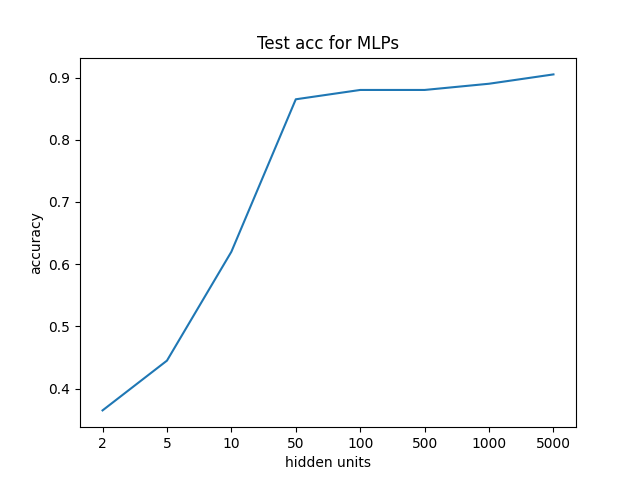
\includegraphics[width=0.65\textwidth]{2_cluster_test_acc.png}
\caption{How test accuracy changes as the hidden layer width increases.}
\end{figure}

\subsection*{3. Analysis and Observations}

\begin{enumerate}
\item \textbf{Under-capacity regime ($n \le 10$).}
When the hidden layer is very small, the network lacks the representational power to capture the non-linear boundary between the two clusters. With just 2 hidden units, accuracy is only 36.5\%, barely above random chance for a two-class problem. At $n=10$, accuracy reaches 62\%, suggesting the model begins to approximate a curved boundary but still misclassifies many points near the border.

\item \textbf{Transition region ($10 < n \le 50$).}
A sharp accuracy jump from 62\% to 86.5\% occurs between $n=10$ and $n=50$. This suggests a phase transition where sufficient hidden units allow the ReLU network to construct a piecewise-linear boundary that closely follows the true data distribution. The improvement of nearly 25 percentage points in this range is the largest single-step gain observed.

\item \textbf{Saturation regime ($n > 50$).}
Beyond 50 hidden units, improvements are incremental: 86.5\% at $n=50$ versus 90.5\% at $n=5000$. Each doubling of capacity yields diminishing marginal gains. The accuracy appears to asymptotically approach an upper bound, likely determined by inherent noise or overlap in the dataset rather than model capacity.

\item \textbf{Decision boundary evolution.}
Visual inspection of the boundaries confirms the quantitative findings. Small networks produce boundaries that are almost straight lines. Medium-sized networks generate smooth curves. Large networks produce highly non-linear, intricate boundaries that wrap tightly around individual data points, indicating the model memorizes fine-grained structure.

\item \textbf{Generalization behavior.}
Despite the extreme over-parameterization at $n=5000$ (10,002 trainable parameters for 800 training samples), test accuracy continues to improve slightly. This aligns with recent theoretical findings that over-parameterized neural networks trained with gradient descent can generalize well even without explicit regularization, particularly in early training regimes (30 epochs here).
\end{enumerate}

\subsection*{4. Selected Decision Boundaries}

\begin{figure}[H]
\centering
\begin{minipage}{0.48\textwidth}
\centering
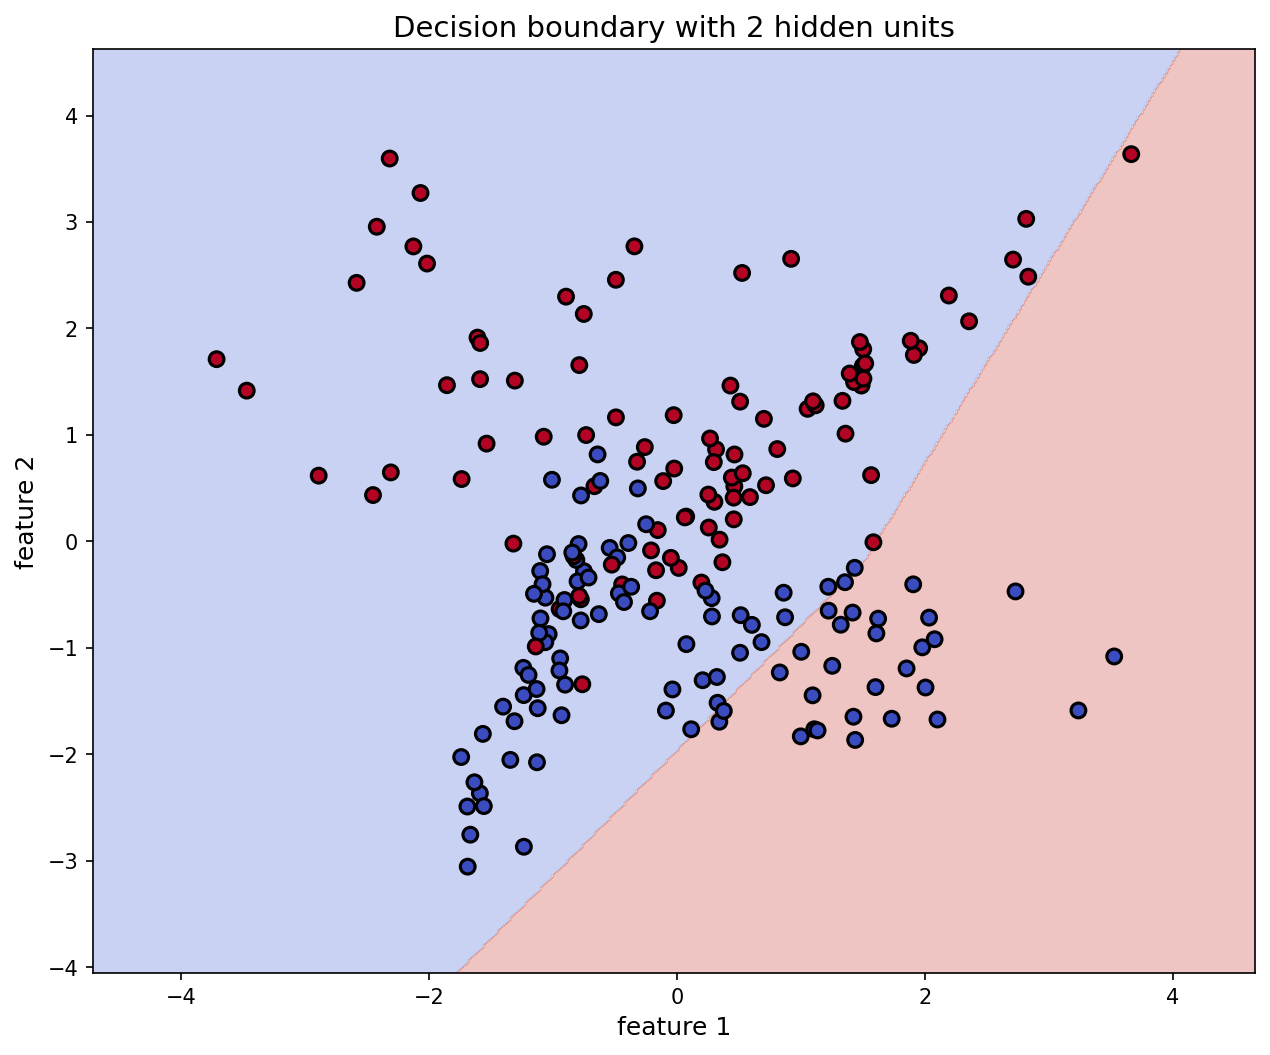
\includegraphics[width=\textwidth]{decision_boundary_2.png}
\caption{$n=2$: near-linear boundary}
\end{minipage}\hfill
\begin{minipage}{0.48\textwidth}
\centering
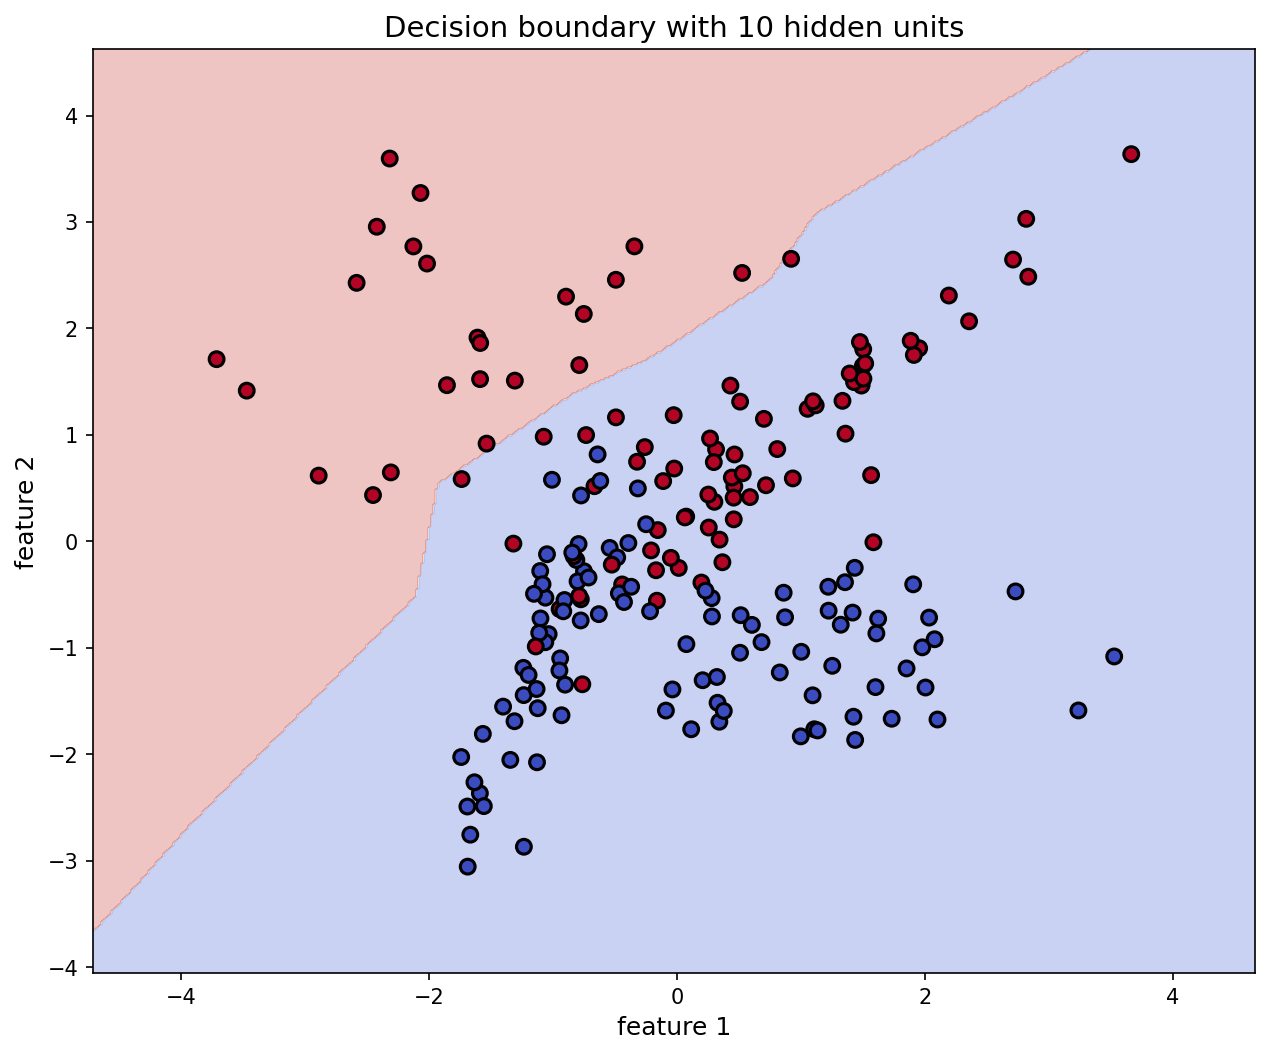
\includegraphics[width=\textwidth]{decision_boundary_10.png}
\caption{$n=10$: curved but rough}
\end{minipage}
\end{figure}

\begin{figure}[H]
\centering
\begin{minipage}{0.48\textwidth}
\centering
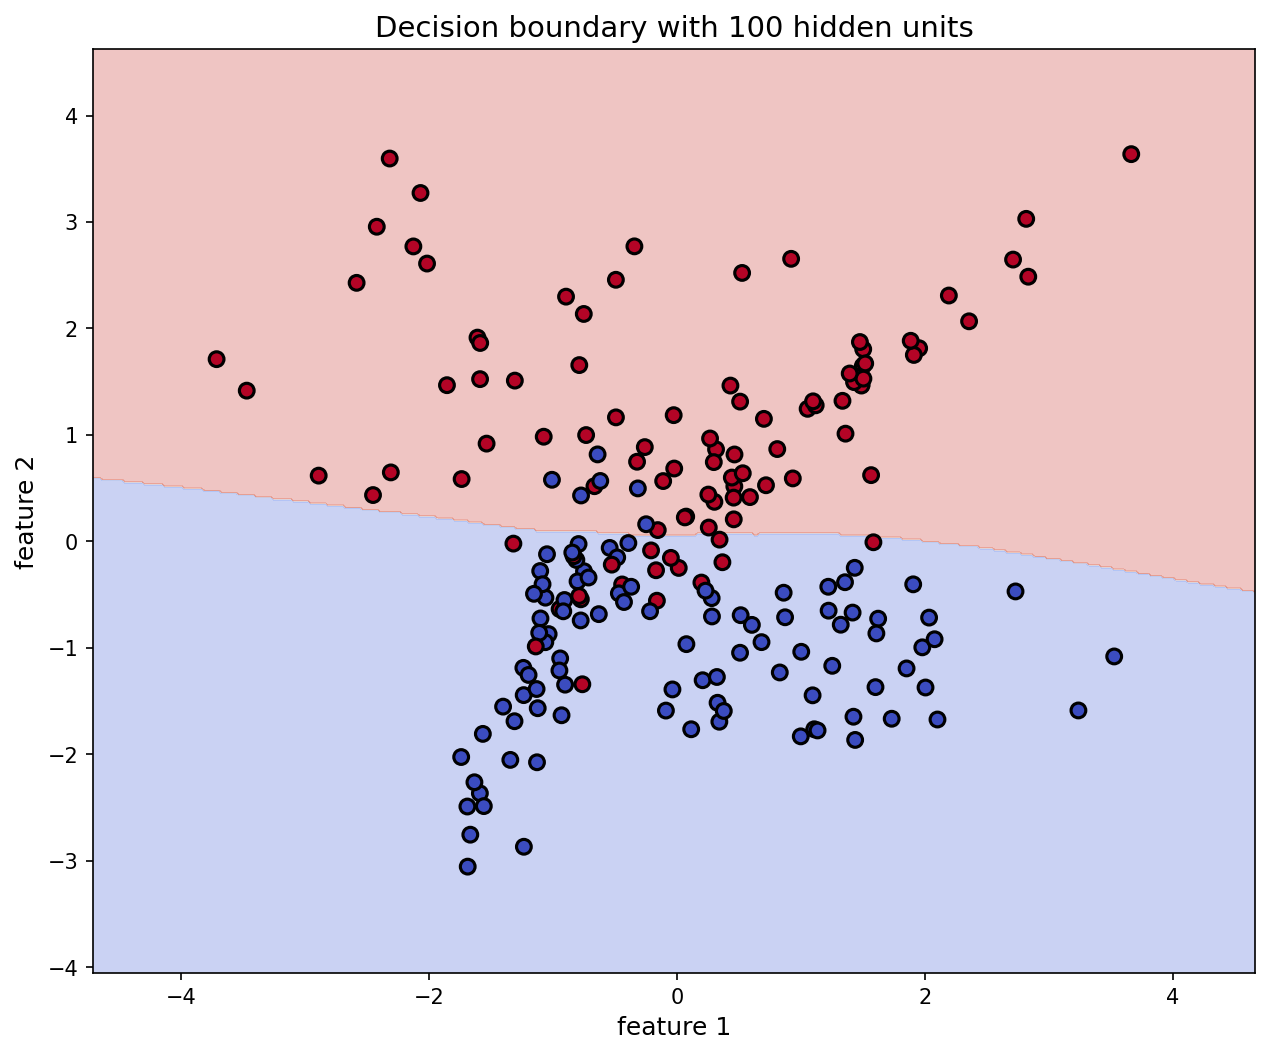
\includegraphics[width=\textwidth]{decision_boundary_100.png}
\caption{$n=100$: smooth non-linear}
\end{minipage}\hfill
\begin{minipage}{0.48\textwidth}
\centering
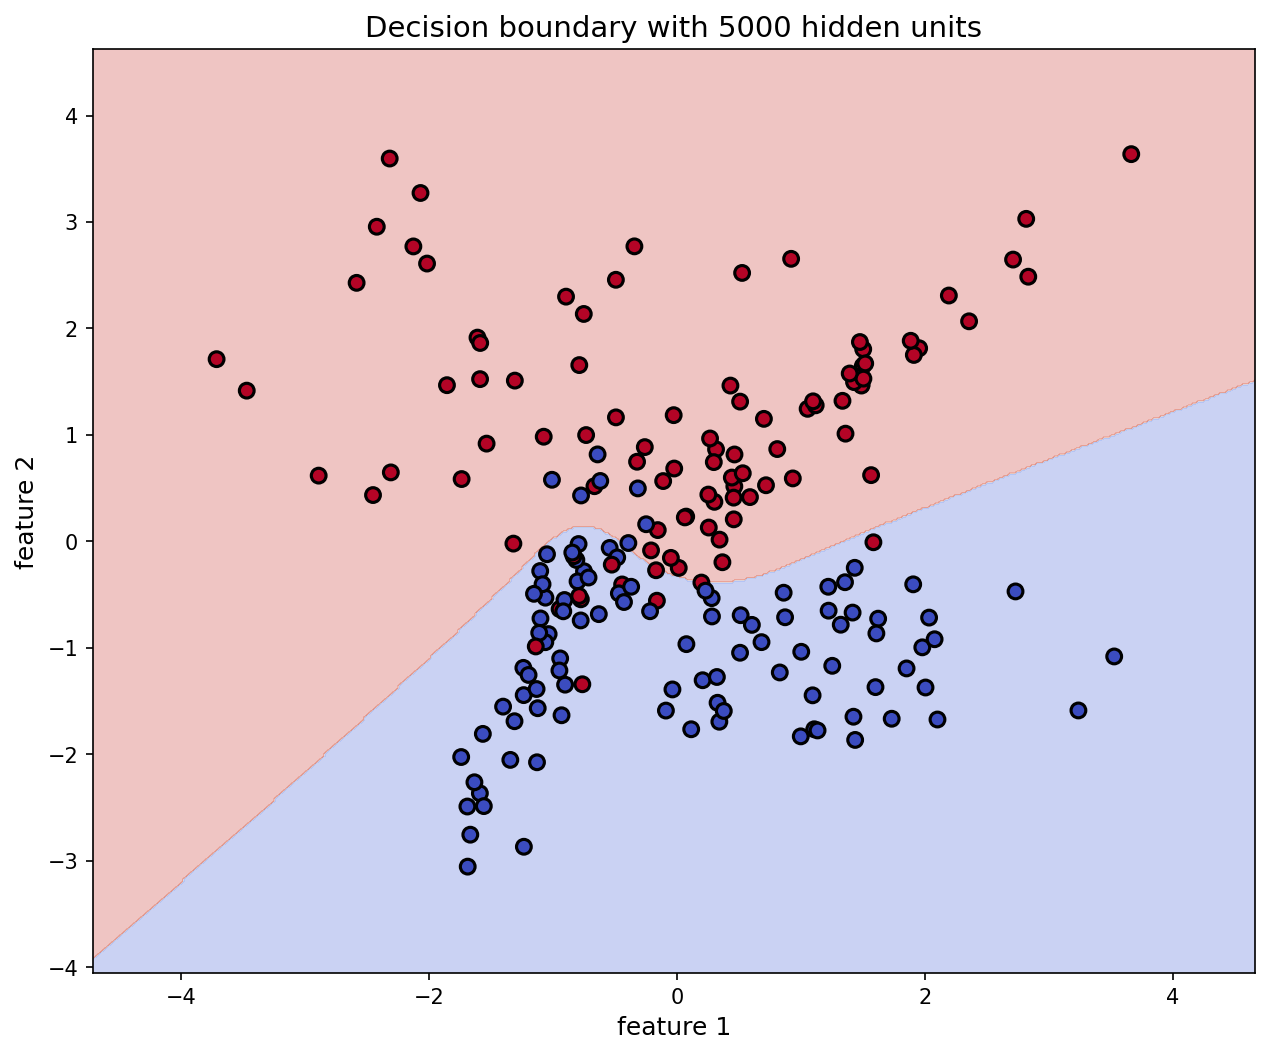
\includegraphics[width=\textwidth]{decision_boundary_5000.png}
\caption{$n=5000$: highly detailed}
\end{minipage}
\end{figure}

\end{Solution}

\end{document}
